% XCircuit output "CF.tex" for LaTeX input from CF.ps
\def\putbox#1#2#3#4{\makebox[0in][l]{\makebox[#1][l]{}\raisebox{\baselineskip}[0in][0in]{\raisebox{#2}[0in][0in]{\scalebox{#3}{#4}}}}}
\def\rightbox#1{\makebox[0in][r]{#1}}
\def\centbox#1{\makebox[0in]{#1}}
\def\topbox#1{\raisebox{-0.60\baselineskip}[0in][0in]{#1}}
\def\midbox#1{\raisebox{-0.20\baselineskip}[0in][0in]{#1}}
   \scalebox{1}{
   \normalsize
   \parbox{2.27604in}{
   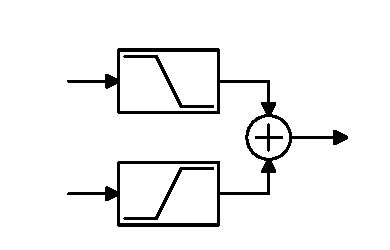
\includegraphics[scale=1]{CF}\\
   % translate x=376 y=304 scale 0.38
   \putbox{1.01in}{1.26in}{1.20}{\centbox{LPF}}%
   \putbox{1.01in}{0.51in}{1.20}{\centbox{HPF}}%
   \putbox{0.35in}{1.12in}{1.20}{\centbox{\midbox{$x_1$}}}%
   \putbox{0.35in}{0.39in}{1.20}{\centbox{\midbox{$x_2$}}}%
   \putbox{2.16in}{0.81in}{1.20}{\centbox{\midbox{$y$}}}%
   } % close 'parbox'
   } % close 'scalebox'
   \vspace{-\baselineskip} % this is not necessary, but looks better
